\documentclass[bachelor, och, labwork]{shiza}
% параметр - тип обучения - одно из значений:
%    spec     - специальность
%    bachelor - бакалавриат (по умолчанию)
%    master   - магистратура
% параметр - форма обучения - одно из значений:
%    och   - очное (по умолчанию)
%    zaoch - заочное
% параметр - тип работы - одно из значений:
%    referat    - реферат
%    coursework - курсовая работа (по умолчанию)
%    diploma    - дипломная работа
%    pract      - отчет по практике
% параметр - включение шрифта
%    times    - включение шрифта Times New Roman (если установлен)
%               по умолчанию выключен
\usepackage{subfigure}
\usepackage{tikz,pgfplots}
\pgfplotsset{compat=1.5}
\usepackage{float}

%\usepackage{titlesec}
\setcounter{secnumdepth}{4}
%\titleformat{\paragraph}
%{\normalfont\normalsize}{\theparagraph}{1em}{}
%\titlespacing*{\paragraph}
%{35.5pt}{3.25ex plus 1ex minus .2ex}{1.5ex plus .2ex}

\titleformat{\paragraph}[block]
{\hspace{1.25cm}\normalfont}
{\theparagraph}{1ex}{}
\titlespacing{\paragraph}
{0cm}{2ex plus 1ex minus .2ex}{.4ex plus.2ex}

% --------------------------------------------------------------------------%


\usepackage[T2A]{fontenc}
\usepackage[utf8]{inputenc}
\usepackage{graphicx}
\graphicspath{ {./images/} }
\usepackage{tempora}

\usepackage[sort,compress]{cite}
\usepackage{amsmath}
\usepackage{amssymb}
\usepackage{amsthm}
\usepackage{fancyvrb}
\usepackage{listings}
\usepackage{listingsutf8}
\usepackage{longtable}
\usepackage{array}
\usepackage[english,russian]{babel}

% \usepackage[colorlinks=true]{hyperref}
\usepackage{url}

\usepackage{underscore}
\usepackage{setspace}
\usepackage{indentfirst} 
\usepackage{mathtools}
\usepackage{amsfonts}
\usepackage{enumitem}
\usepackage{tikz}

\newcommand{\eqdef}{\stackrel {\rm def}{=}}
\newcommand{\specialcell}[2][c]{%
\begin{tabular}[#1]{@{}c@{}}#2\end{tabular}}

\renewcommand\theFancyVerbLine{\small\arabic{FancyVerbLine}}

\newtheorem{lem}{Лемма}

\begin{document}

% Кафедра (в родительном падеже)
\chair{}

% Тема работы
\title{Сетевая утилита ping}

% Курс
\course{2}

% Группа
\group{231}

% Факультет (в родительном падеже) (по умолчанию "факультета КНиИТ")
\department{факультета КНиИТ}

% Специальность/направление код - наименование
%\napravlenie{09.03.04 "--- Программная инженерия}
%\napravlenie{010500 "--- Математическое обеспечение и администрирование информационных систем}
%\napravlenie{230100 "--- Информатика и вычислительная техника}
%\napravlenie{231000 "--- Программная инженерия}
\napravlenie{100501 "--- Компьютерная безопасность}

% Для студентки. Для работы студента следующая команда не нужна.
% \studenttitle{Студентки}

% Фамилия, имя, отчество в родительном падеже
\author{Окунькова Сергея Викторовича}

% Заведующий кафедрой
% \chtitle{} % степень, звание
% \chname{}

%Научный руководитель (для реферата преподаватель проверяющий работу)
\satitle{ассистент} %должность, степень, звание
\saname{А. А. Фомин}

% Руководитель практики от организации (только для практики,
% для остальных типов работ не используется)
% \patitle{к.ф.-м.н.}
% \paname{С.~В.~Миронов}

% Семестр (только для практики, для остальных
% типов работ не используется)
%\term{8}

% Наименование практики (только для практики, для остальных
% типов работ не используется)
%\practtype{преддипломная}

% Продолжительность практики (количество недель) (только для практики,
% для остальных типов работ не используется)
%\duration{4}

% Даты начала и окончания практики (только для практики, для остальных
% типов работ не используется)
%\practStart{30.04.2019}
%\practFinish{27.05.2019}

% Год выполнения отчета
\date{2021}

\maketitle

% Включение нумерации рисунков, формул и таблиц по разделам
% (по умолчанию - нумерация сквозная)
% (допускается оба вида нумерации)
% \secNumbering

%-------------------------------------------------------------------------------------------


\begin{enumerate}
    
    \item Воспользовавшись командой ping проверьте доступность одного из компьютеров вашего учебного класса.
    
    \begin{figure}[H]
        \centering      %размер рисунка       здесь находится название файла рисунка, без указания формата
        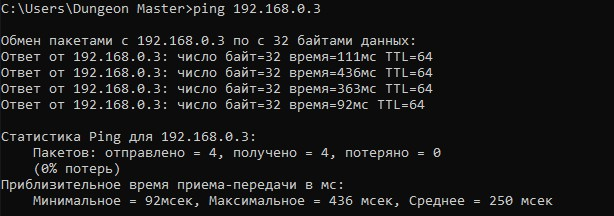
\includegraphics[width=0.75\textwidth]{1}
        \caption{Проверка доступности компьютера командой ping}
        \label{fig:image1}
    \end{figure}

    \item Воспользовавшись командой ping проверьте доступность сервера www.sgu.ru
    
    \begin{figure}[H]
        \centering      %размер рисунка       здесь находится название файла рисунка, без указания формата
        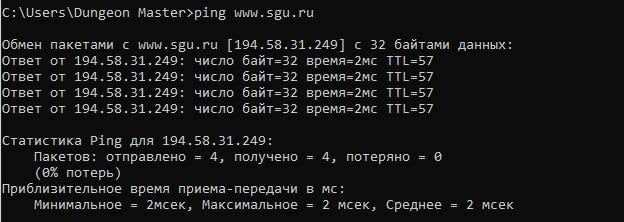
\includegraphics[width=0.75\textwidth]{2}
        \caption{Проверка доступности сервера www.sgu.ru командой ping}
        \label{fig:image1}
    \end{figure}

    \item Воспользуйтесь командой ping с параметром записи маршрута и числом отправляемых сообщений 1 для  www.sgu.ru
    
    \begin{figure}[H]
        \centering      %размер рисунка       здесь находится название файла рисунка, без указания формата
        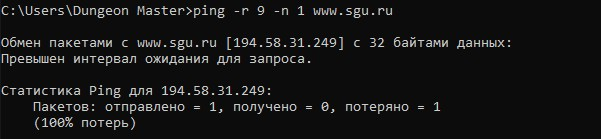
\includegraphics[width=0.75\textwidth]{3}
        \caption{Проверка доступности сервера www.sgu.ru командой ping с параметром записи маршрута и числом отправляемых сообщений}
        \label{fig:image1}
    \end{figure}

    \item Проделайте то же для любого внешнего www сервера на ваш выбор.
    
    \begin{figure}[H]
        \centering      %размер рисунка       здесь находится название файла рисунка, без указания формата
        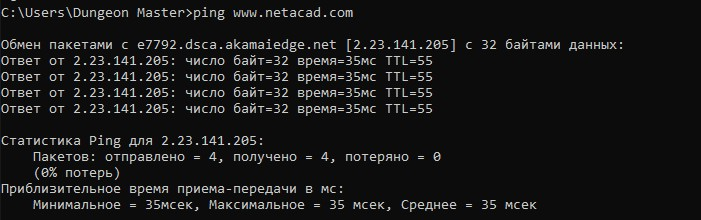
\includegraphics[width=0.75\textwidth]{4}
        \caption{Проверка доступности сервера www.netacad.com командой ping}
        \label{fig:image1}
    \end{figure}

    \begin{figure}[H]
        \centering      %размер рисунка       здесь находится название файла рисунка, без указания формата
        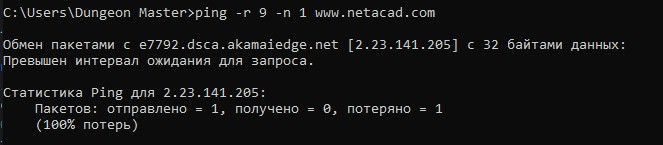
\includegraphics[width=0.75\textwidth]{5}
        \caption{Проверка доступности сервера www.netacad.com командой ping с параметром записи маршрута и числом отправляемых сообщений}
        \label{fig:image1}
    \end{figure}

    \item Продемонстрируйте использование опции разрешения ip- адреса в доменное имя.
    
    \begin{figure}[H]
        \centering      %размер рисунка       здесь находится название файла рисунка, без указания формата
        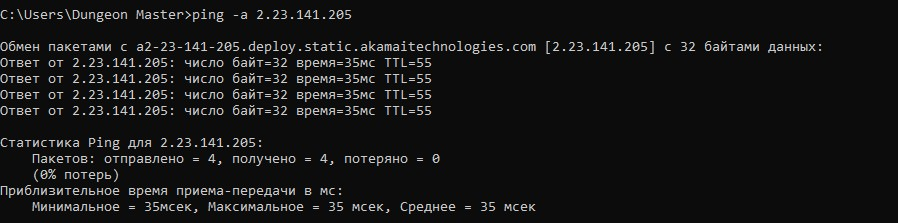
\includegraphics[width=0.75\textwidth]{6}
        \caption{Пример использование опции разрешения ip- адреса в доменное имя}
        \label{fig:image1}
    \end{figure}

    \item Установив параметр «число отправляемых сообщений» равным 2, проверьте прохождение пакетов до выбранного узла при увеличении 
    длины отправляемых пакетов (увеличивая длину пакета каждый раз в 2 раза).

    \begin{figure}[H]
        \centering      %размер рисунка       здесь находится название файла рисунка, без указания формата
        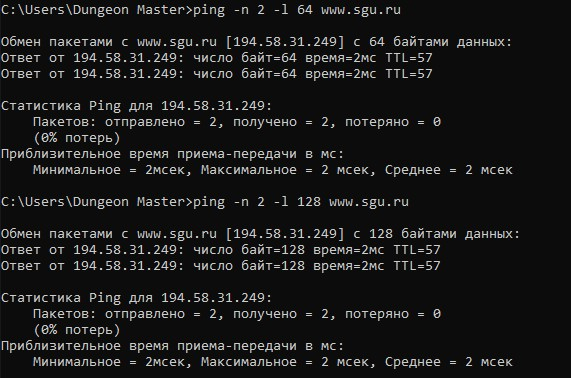
\includegraphics[width=0.75\textwidth]{7}
        \caption{Прохождение пакетов при длине пакетов 64 и 128}
        \label{fig:image1}
    \end{figure}

    \begin{figure}[H]
        \centering      %размер рисунка       здесь находится название файла рисунка, без указания формата
        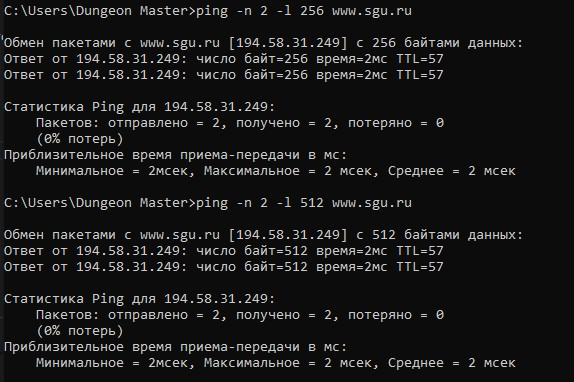
\includegraphics[width=0.75\textwidth]{8}
        \caption{Прохождение пакетов при длине пакетов 256 и 512}
        \label{fig:image1}
    \end{figure}

    \begin{figure}[H]
        \centering      %размер рисунка       здесь находится название файла рисунка, без указания формата
        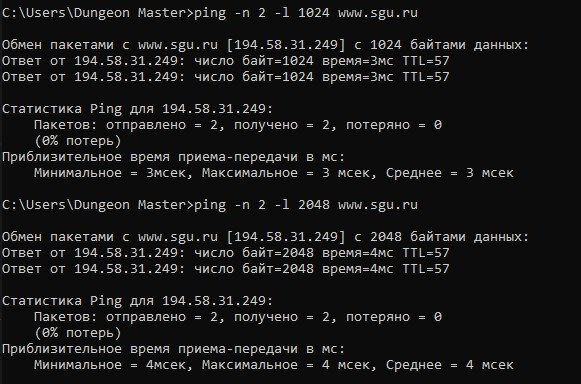
\includegraphics[width=0.75\textwidth]{9}
        \caption{Прохождение пакетов при длине пакетов 1024 и 2048}
        \label{fig:image1}
    \end{figure}

    \begin{figure}[H]
        \centering      %размер рисунка       здесь находится название файла рисунка, без указания формата
        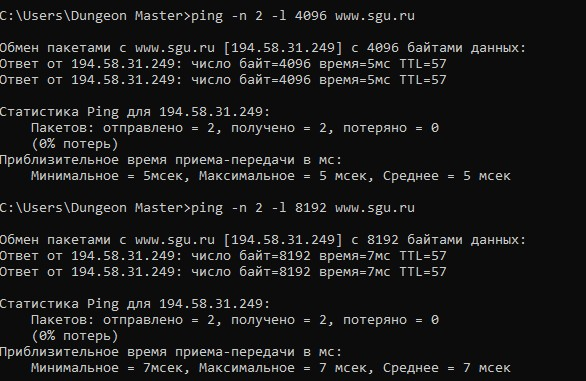
\includegraphics[width=0.75\textwidth]{10}
        \caption{Прохождение пакетов при длине пакетов 4096 и 8192}
        \label{fig:image1}
    \end{figure}

    \begin{figure}[H]
        \centering      %размер рисунка       здесь находится название файла рисунка, без указания формата
        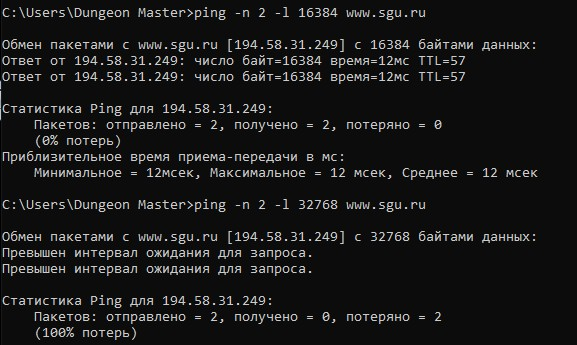
\includegraphics[width=0.75\textwidth]{11}
        \caption{Прохождение пакетов при длине пакетов 16384 и 32768}
        \label{fig:image1}
    \end{figure}

    \item Повторите предыдущее задание с установленным флагом запрещения фрагментации. Сопоставьте и объясните результаты.
    
    Если мы установим флаг запрещающий фрагментацию, то результат начнет менятся только со значения 2048, так как для 
    передачи пакетов такой длины нужна фрагментация, а у нас стоит флаг запрещающий ее.

    \begin{figure}[H]
        \centering      %размер рисунка       здесь находится название файла рисунка, без указания формата
        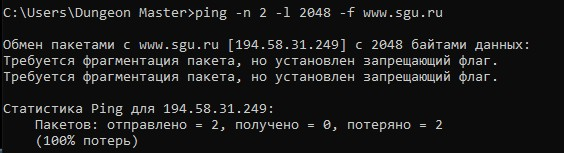
\includegraphics[width=0.75\textwidth]{12}
        \caption{Результат команды ping про запрещающем фрагментацию флаге и длине пакетов 2048}
        \label{fig:image1}
    \end{figure}

\end{enumerate}

\end{document}
